\chapter{Měření srážek}

\section{Požadavky}

Srážkoměr bude součástí venkovního modulu, takže musí fungovat dlouhodobě venku a~jeho signál musí zpracovat mikrokontrolér. Naměřená data se použijí pro 15minutové souhrny, pro denní a~týdenní přehled srážek a~pro jednoduché doporučení zálivky, proto musí být měření stabilní a~opakovatelné. Zařízení se musí dát snadno zapojit a~naprogramovat, mělo by jít objednat z~evropského obchodu a~výhodou je také dostupná dokumentace.

\section{Principy měření}

\subsection{Kyvný kyblík}

Nejrozšířenějším principem je kyvný kyblík (anglicky \textit{tipping bucket}). Voda ze sběrné nálevky teče do kyvné nádobky se dvěma komorami. Jakmile se jedna komora naplní na určitý objem, nádobka se převrátí, voda vyteče a~plnit se začne druhá komora. Při každém převrácení se pomocí magnetu sepne jazýčkový kontakt, který vytvoří jeden impuls. Jeden impuls tak odpovídá pevně dané výšce srážek. U~srážkoměrů pro malé meteostanice to je například 0,2794~mm na jedno překlopení~\cite{sparkfun}, jiný výrobce ale uvádí 0,3~mm~\cite{misol}.

Princip je znázorněn na obrázku~\ref{fig:kyblik}.

\begin{figure}[htbp]
\centering
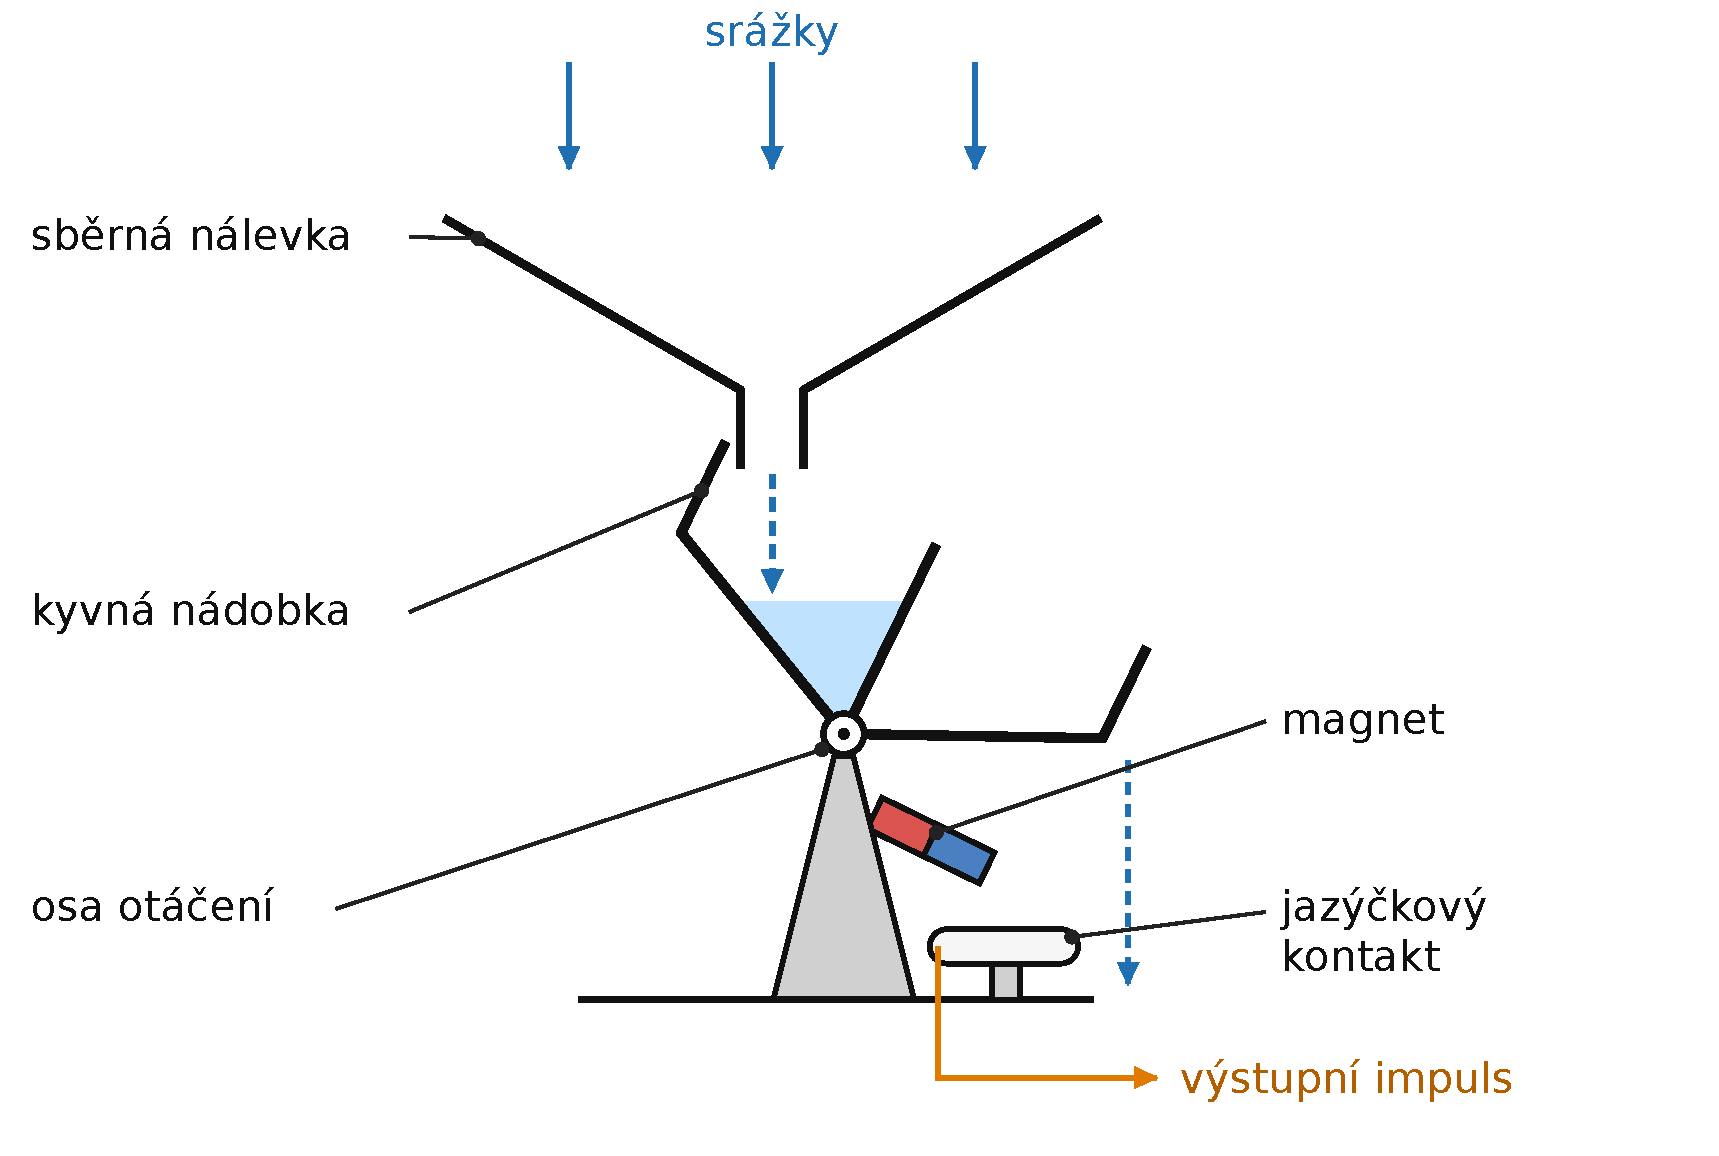
\includegraphics[width=0.8\textwidth]{kyvny_kyblik}
\caption{Princip srážkoměru s~kyvným kyblíkem}
\label{fig:kyblik}
\end{figure}

Výstup je pro mikrokontrolér velmi jednoduchý. Kontakt neobsahuje žádnou aktivní elektroniku a~stačí ho připojit na vstup s~přerušením a~počítat impulsy~\cite{sparkfun}. Tímto způsobem je řešený například srážkoměr v~diplomové práci o~domácí meteostanici, kde mikrokontrolér ESP32 počítá překlopení v~přerušení~\cite{macek}. Základní provedení srážkoměru není vytápěné, takže měří jen kapalné srážky, vytápění umožňuje měřit i sníh~\cite{macek}.

\subsection{Váhový princip}

Při váhovém principu se voda zachycuje do nádoby a~její hmotnost se měří snímačem síly. Výška srážek se dopočítá z~hmotnosti vody a~plochy nálevky, protože 1~mm srážek odpovídá 1~kg vody na metr čtvereční. Při sběrné ploše 200~cm$^2$ tedy 1~mm srážek odpovídá 20~g vody a~0,2~mm odpovídá 4~g. Typickým profesionálním příkladem je OTT Pluvio$^2$ S, který váží uzavřeným snímačem síly, má sběrnou plochu 200~cm$^2$, kapacitu 400~mm a~přesnost $\pm$0,1~mm nebo $\pm$1~\% naměřené hodnoty. Váží kolem 7,8~kg a~je určený pro profesionální použití~\cite{ott}.

Jako možnost vlastní stavby by šlo postavit váhový srážkoměr s~tenzometrickým snímačem. Voda z~nálevky by se zachytávala do nádoby, jejíž hmotnost by se měřila a~digitalizovala 24bitovým převodníkem HX711~\cite{hx711}. Nádoba by se vyprazdňovala posuvným šoupátkem poháněným servem. U~takového konceptu je potřeba řešit vyprazdňování nádoby tak, aby nezkreslovalo vážení, a~počítat také s~pohybem konstrukce při větru.

Koncept je znázorněn na obrázku~\ref{fig:vahovy}.

\begin{figure}[htbp]
\centering
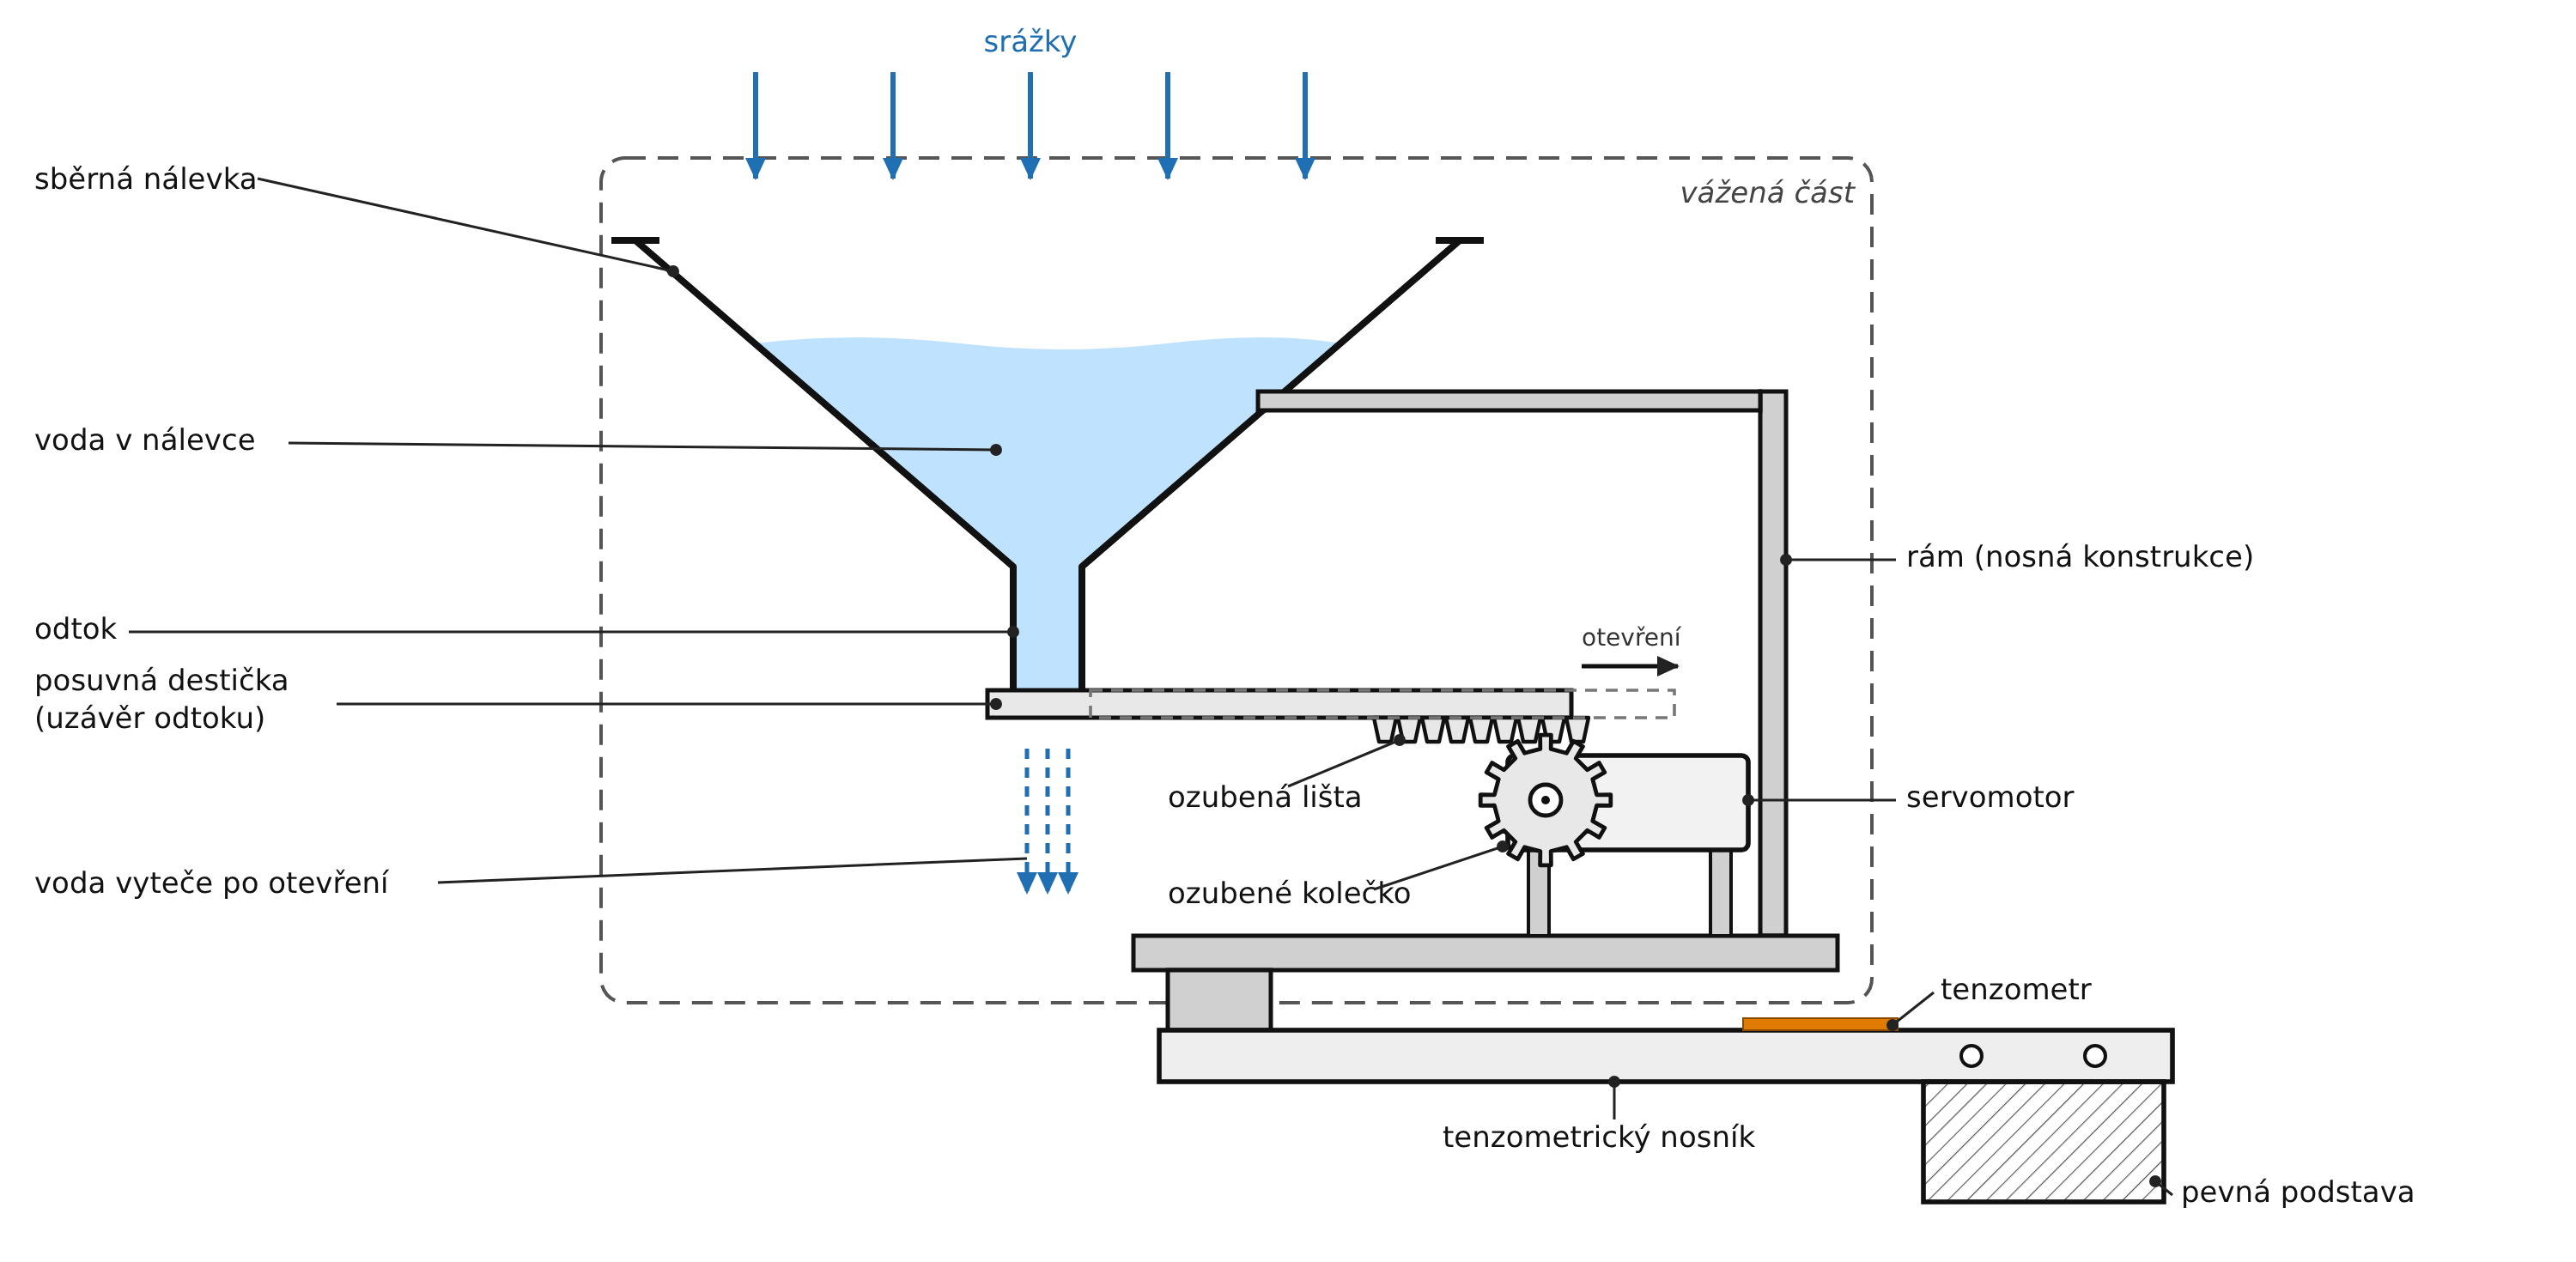
\includegraphics[width=\textwidth]{vahovy_srazkomer}
\caption{Koncept váhového srážkoměru s~tenzometrem}
\label{fig:vahovy}
\end{figure}

\subsection{Optické a~další principy}

Optický srážkoměr nesbírá vodu, ale srážky odhaduje. Infračervené světlo se uvnitř čočky odráží k~detektorům a~kapky dopadající na povrch čočky způsobí, že část světla uniká ven. Z~poklesu intenzity se odhadne velikost kapek a~z~nich množství srážek~\cite{cnx}. Příkladem je Hydreon RG-15, který nemá žádné pohyblivé části. V~klidu spotřebuje asi 110~$\mu$A, za deště 2 až 4~mA. Jeho výstup napodobuje kyblík a~je k~dispozici i~sériové rozhraní. Nominální přesnost je $\pm$10~\%, výrobce uvádí, že se v~terénu může lišit, a~při mrznoucím dešti senzor srážky nezaznamená~\cite{rg15}. Existují i~další principy, například piezoelektrické nebo radarové, ty se ale používají hlavně v~komplexnějších čidlech.

\section{Porovnání principů}

Tabulka~\ref{tab:srazky} shrnuje hlavní vlastnosti popsaných principů a~konkrétních řešení.

\newcolumntype{Y}[1]{>{\hsize=#1\hsize\raggedright\arraybackslash}X}

\begin{center}
\noindent\begin{minipage}{\textwidth}
\captionof{table}{Porovnání principů a~konkrétních řešení měření srážek}
\label{tab:srazky}
\scriptsize
\renewcommand{\arraystretch}{1.25}
\begin{tabularx}{\textwidth}{|Y{1.5}|Y{0.8}|Y{0.8}|Y{0.9}|}
\hline
\textbf{Řešení} & \textbf{Rozlišení} & \textbf{Přesnost} & \textbf{Výstup} \\
\hline
\rowcolor{gray!15}\multicolumn{4}{|l|}{\textbf{Kyvný kyblík}} \\
\hline
HESTORE WH-SP-RG (plast) & 0,2794~mm & $\pm$5~\% & kontakt \\
\hline
Davis 6466M (UV-ABS) & 0,2~mm & $\pm$3~\% & kontakt \\
\hline
Rika RK400-01 (nerez, ABS) & 0,2~mm & $\pm$4~\% & kontakt, RS485 \\
\hline
Veinasa XS-RS04 (nerez) & 0,2~mm & $\pm$4~\% & kontakt \\
\hline
BGT WS-601 SS (nerez) & 0,2~mm & $\pm$2~\% & kontakt, RS485 \\
\hline
\rowcolor{gray!15}\multicolumn{4}{|l|}{\textbf{Váhový}} \\
\hline
OTT Pluvio$^2$ S (7,8~kg) & 0,05 až 0,2~mm & $\pm$1~\% & impulsy, SDI-12, RS-485 \\
\hline
Vlastní koncept (tenzometr, HX711) & dáno snímačem & neověřena & HX711 \\
\hline
\rowcolor{gray!15}\multicolumn{4}{|l|}{\textbf{Optický}} \\
\hline
Hydreon RG-15 & 0,2~mm & $\pm$10~\% & open-collector, UART \\
\hline
Renke Optical Rain Gauge & 0,1~mm & $\pm$5~\% & RS485, impulsy \\
\hline
\end{tabularx}

\vspace{0.3em}
{\scriptsize
Poznámky: přesnost je podle výrobce. U~Davisu je to $\pm$3~\% nebo jedno překlopení, u~Riky a~Veinasy $\pm$4~\% při testu uvnitř při 2~mm/min, u~BGT $\pm$2~\% do 240~mm/h a~u~OTT $\pm$0,1~mm nebo $\pm$1~\%. Zdroje:~\cite{hestore,sparkfun,misol,davis,rika,veinasa,bgt,ott,rg15,renkeopt}.\par}
\end{minipage}
\end{center}

\chapter{Měření větru}

\section{Požadavky}

Venkovní modul má měřit rychlost i~směr větru. Čidlo musí být určené pro venkovní použití, mít co nejjednodušší výstup, který zvládne přečíst mikrokontrolér bez dalších obvodů, a~hlavně musí mít dostupnou dokumentaci. Podle ní poznám, co přesně čidlo měří a~jak ho zapojit.

\section{Principy měření}

\subsection{Miskový anemometr}

Nejběžnější je miskový anemometr. Vítr roztáčí tři nebo čtyři misky na svislé ose a~na ose je magnet. Ten při každé otáčce sepne jazýčkový kontakt (reed) nebo ho zaznamená Hallova sonda. Mikrokontrolér počítá impulsy za určitý čas a~z~jejich frekvence spočítá rychlost. U~čidel typu Fine Offset a~Misol odpovídá jedno sepnutí za sekundu rychlosti 2,4~km/h~\cite{sparkfun}. Výstup je čistě digitální, takže stačí jeden vstup s~počítáním impulsů.

Princip je znázorněn na obrázku~\ref{fig:anemometr}.

\begin{figure}[htbp]
\centering
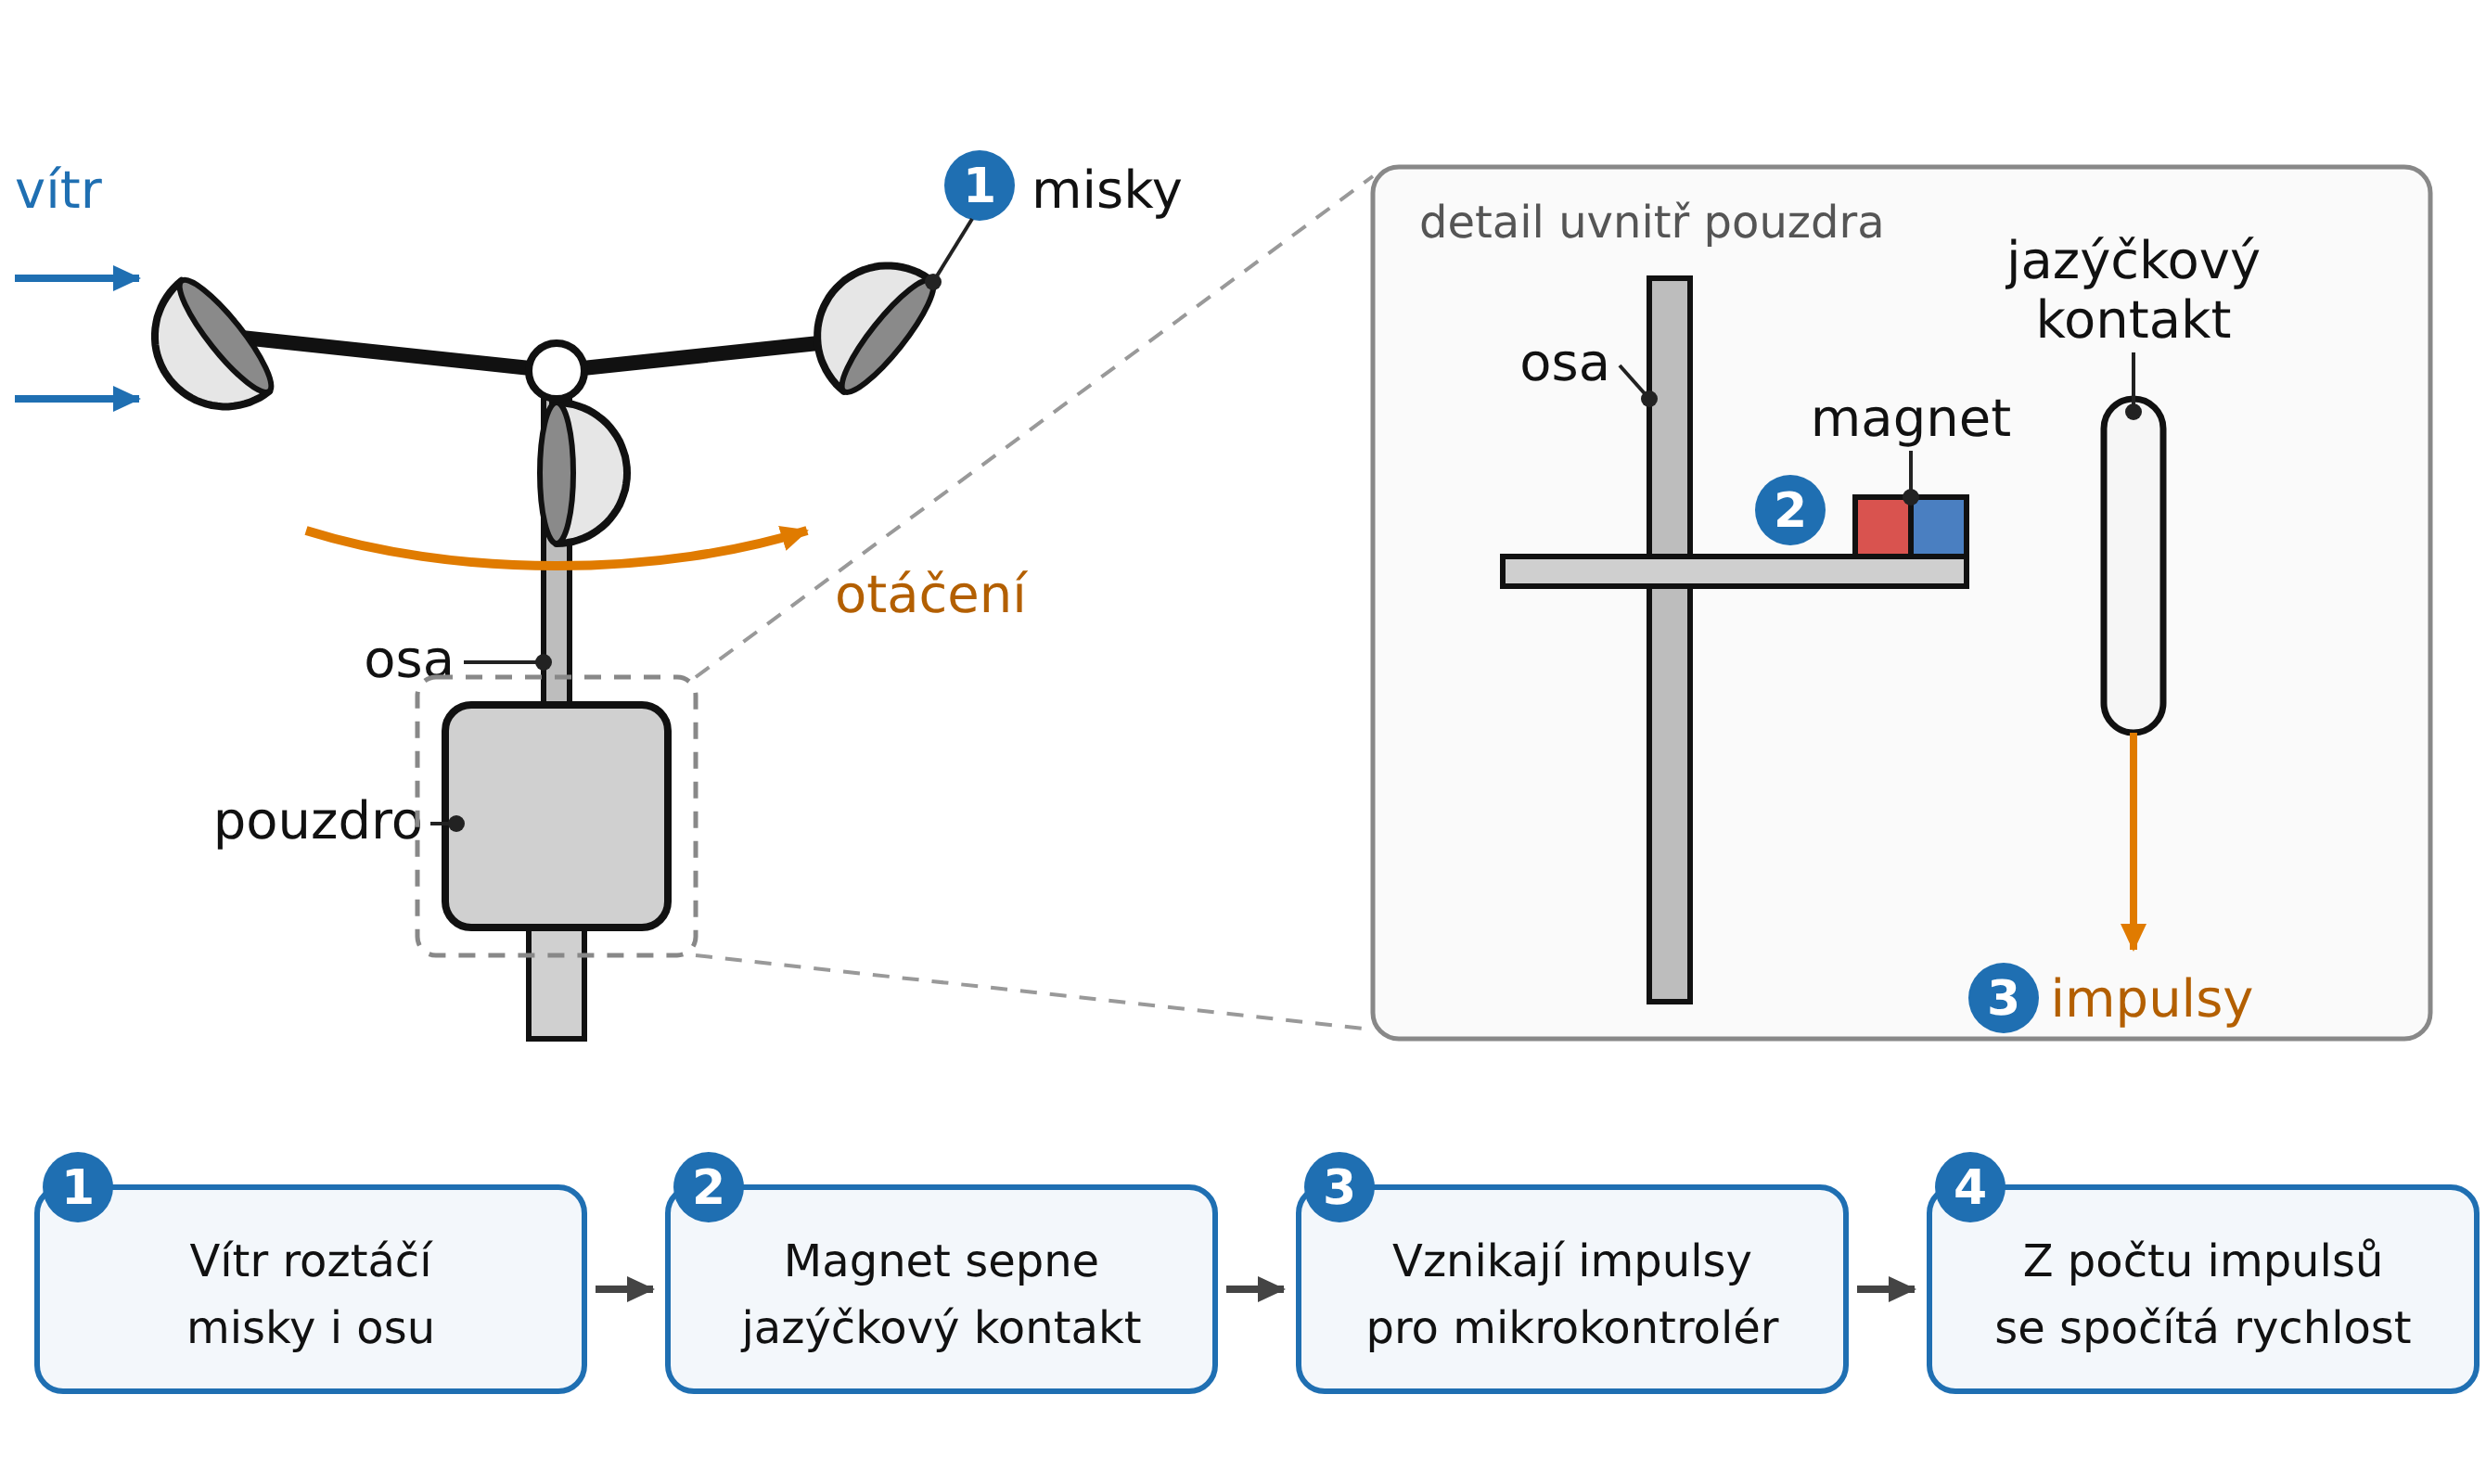
\includegraphics[width=\textwidth]{miskovy_anemometr}
\caption{Princip miskového anemometru}
\label{fig:anemometr}
\end{figure}

\subsection{Větrná směrovka}

Směrovka se otáčí podle směru větru a~nese magnet. Kolem osy je osm jazýčkových kontaktů, z~nichž každý je zapojený s~jiným odporem. Magnet může sepnout jeden kontakt nebo dva sousední najednou, takže vznikne 16~poloh~\cite{sparkfun}. Každá poloha dá na odporovém děliči jiné napětí. To se přečte analogovým vstupem mikrokontroléru a~podle změřené hodnoty se přiřadí ke směru. Dražší čidla používají jiné způsoby snímání a~směr udávají přímo ve stupních.

Princip je znázorněn na obrázku~\ref{fig:smerovka}.

\begin{figure}[htbp]
\centering
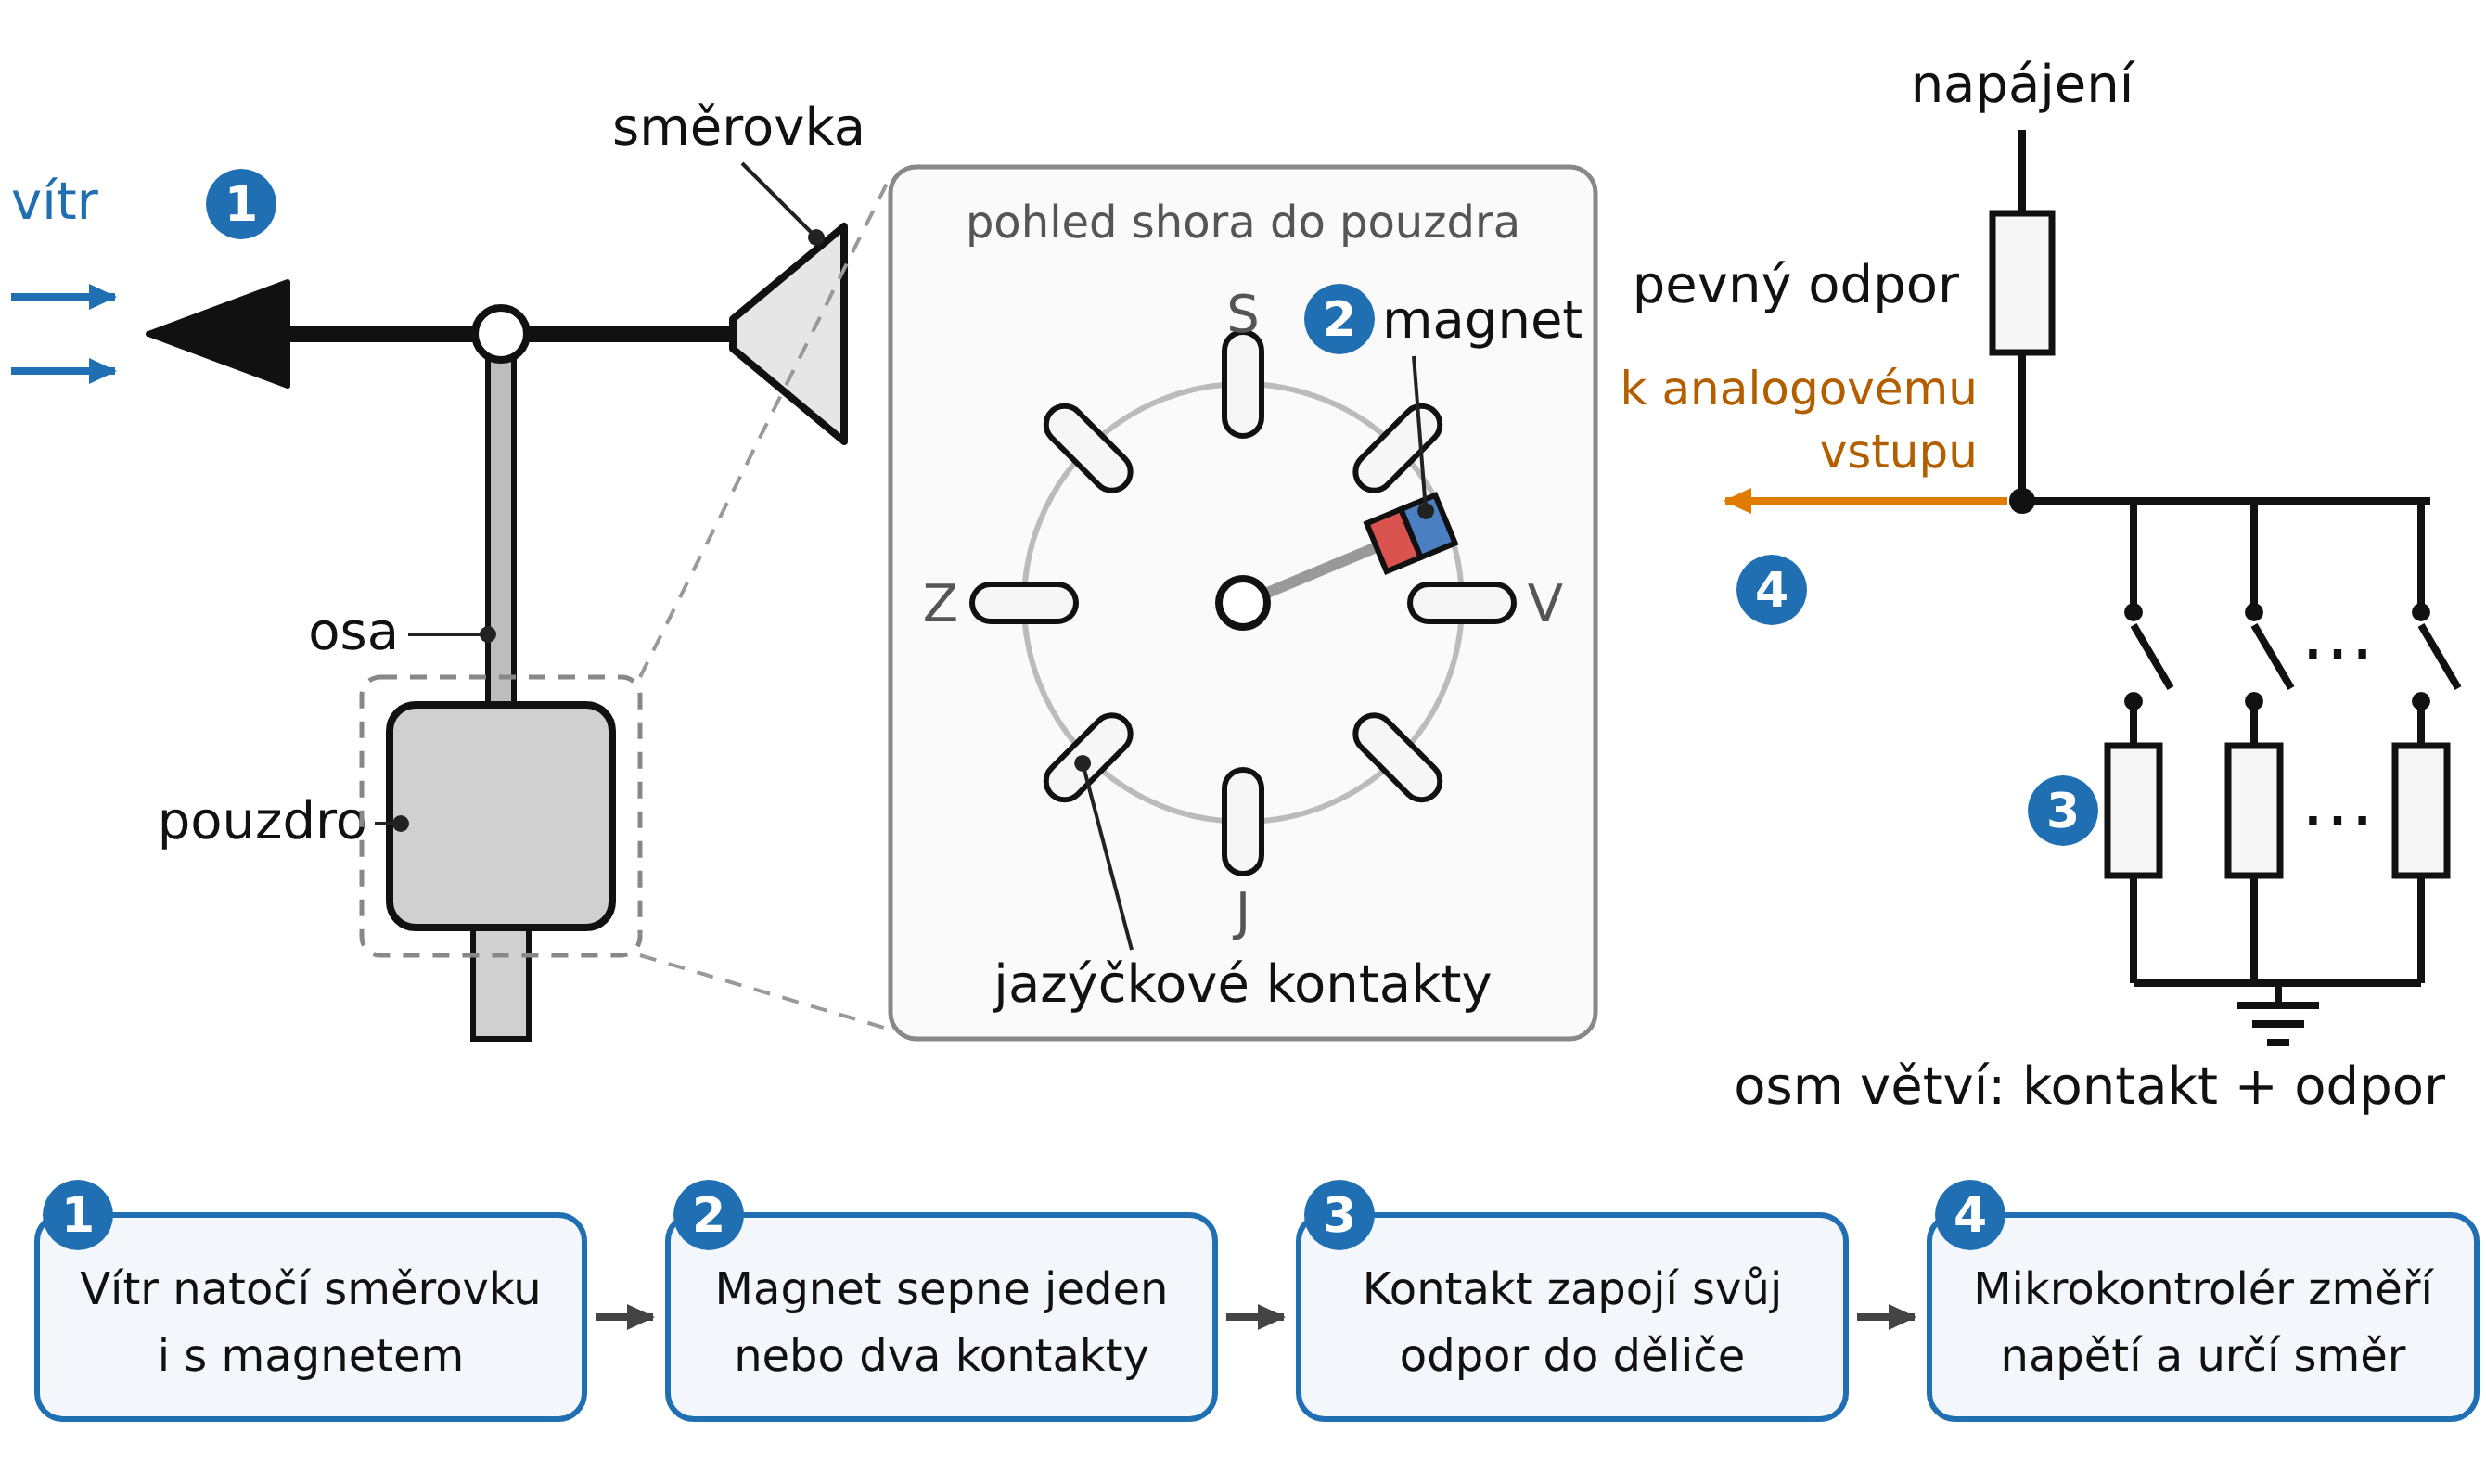
\includegraphics[width=\textwidth]{vetrna_smerovka}
\caption{Princip větrné směrovky s~jazýčkovými kontakty}
\label{fig:smerovka}
\end{figure}

\subsection{Ultrazvukový anemometr}

Ultrazvukový anemometr nemá žádné pohyblivé části. Mezi několika páry měničů posílá krátké ultrazvukové pulzy a~měří, o~kolik se změní doba letu proti větru a~po větru. Z~rozdílu časů se spočítá rychlost i~směr najednou. Výstup bývá digitální, takže je potřeba řešit i~komunikaci s~čidlem.

\subsection{Vrtulkový anemometr}

Vrtulkový anemometr má vrtuli na vodorovné ose a~otáčí se proti větru, takže měří rychlost i~směr jedním čidlem. Používá se hlavně u~profesionálních stanic a~na letištích, proto se mu dál nevěnuji.

\section{Porovnání řešení}

Tabulka~\ref{tab:vitr} shrnuje tři řešení, ke kterým jsem našel dokumentaci. Údaje jsou převzaté z~katalogů a~datasheetů výrobců.

\begin{center}
\noindent\begin{minipage}{\textwidth}
\captionof{table}{Porovnání konkrétních řešení měření větru}
\label{tab:vitr}
\scriptsize
\renewcommand{\arraystretch}{1.25}
\begin{tabularx}{\textwidth}{|Y{1.2}|Y{0.8}|Y{1.1}|Y{0.9}|}
\hline
\textbf{Řešení} & \textbf{Rozsah} & \textbf{Přesnost} & \textbf{Výstup} \\
\hline
\rowcolor{gray!15}\multicolumn{4}{|l|}{\textbf{Miskový anemometr a~směrovka}} \\
\hline
Fine Offset / Misol (anemometr + směrovka) & 0 až 50~m/s & $\pm$1~m/s do 10~m/s, nad tím $\pm$10~\% & kontakt, odporový dělič \\
\hline
Rika RK100-01 + RK110-01 & 0 až 30~m/s & $\pm(0{,}3+0{,}03\,V)$~m/s, směr $\pm$3$^\circ$ & impulsy, napětí, 4--20~mA, RS485 \\
\hline
\rowcolor{gray!15}\multicolumn{4}{|l|}{\textbf{Ultrazvukový}} \\
\hline
Calypso ULP & 0 až 25 nebo 0 až 45~m/s & 1~\% při 10~m/s, směr $\pm$1$^\circ$ & sériový výstup, Modbus \\
\hline
\end{tabularx}

\vspace{0.3em}
{\scriptsize
Poznámky: rozsah a~přesnost u~Fine Offset jsou údaje výrobce pro jeho stanici WH3080, která používá stejný typ čidel. U~Riky je $V$ naměřená rychlost větru v~m/s. Zdroje:~\cite{fineoffset,misolwd,rikawind,rikadir,calypso}.\par}
\end{minipage}
\end{center}